% Options for packages loaded elsewhere
\PassOptionsToPackage{unicode}{hyperref}
\PassOptionsToPackage{hyphens}{url}
%
\documentclass[
]{article}
\usepackage{lmodern}
\usepackage{amssymb,amsmath}
\usepackage{ifxetex,ifluatex}
\ifnum 0\ifxetex 1\fi\ifluatex 1\fi=0 % if pdftex
  \usepackage[T1]{fontenc}
  \usepackage[utf8]{inputenc}
  \usepackage{textcomp} % provide euro and other symbols
\else % if luatex or xetex
  \usepackage{unicode-math}
  \defaultfontfeatures{Scale=MatchLowercase}
  \defaultfontfeatures[\rmfamily]{Ligatures=TeX,Scale=1}
\fi
% Use upquote if available, for straight quotes in verbatim environments
\IfFileExists{upquote.sty}{\usepackage{upquote}}{}
\IfFileExists{microtype.sty}{% use microtype if available
  \usepackage[]{microtype}
  \UseMicrotypeSet[protrusion]{basicmath} % disable protrusion for tt fonts
}{}
\makeatletter
\@ifundefined{KOMAClassName}{% if non-KOMA class
  \IfFileExists{parskip.sty}{%
    \usepackage{parskip}
  }{% else
    \setlength{\parindent}{0pt}
    \setlength{\parskip}{6pt plus 2pt minus 1pt}}
}{% if KOMA class
  \KOMAoptions{parskip=half}}
\makeatother
\usepackage{xcolor}
\IfFileExists{xurl.sty}{\usepackage{xurl}}{} % add URL line breaks if available
\IfFileExists{bookmark.sty}{\usepackage{bookmark}}{\usepackage{hyperref}}
\hypersetup{
  pdftitle={AIR Data Analysis Q1},
  pdfauthor={Leonid Rempel},
  hidelinks,
  pdfcreator={LaTeX via pandoc}}
\urlstyle{same} % disable monospaced font for URLs
\usepackage[margin=1in]{geometry}
\usepackage{color}
\usepackage{fancyvrb}
\newcommand{\VerbBar}{|}
\newcommand{\VERB}{\Verb[commandchars=\\\{\}]}
\DefineVerbatimEnvironment{Highlighting}{Verbatim}{commandchars=\\\{\}}
% Add ',fontsize=\small' for more characters per line
\usepackage{framed}
\definecolor{shadecolor}{RGB}{248,248,248}
\newenvironment{Shaded}{\begin{snugshade}}{\end{snugshade}}
\newcommand{\AlertTok}[1]{\textcolor[rgb]{0.94,0.16,0.16}{#1}}
\newcommand{\AnnotationTok}[1]{\textcolor[rgb]{0.56,0.35,0.01}{\textbf{\textit{#1}}}}
\newcommand{\AttributeTok}[1]{\textcolor[rgb]{0.77,0.63,0.00}{#1}}
\newcommand{\BaseNTok}[1]{\textcolor[rgb]{0.00,0.00,0.81}{#1}}
\newcommand{\BuiltInTok}[1]{#1}
\newcommand{\CharTok}[1]{\textcolor[rgb]{0.31,0.60,0.02}{#1}}
\newcommand{\CommentTok}[1]{\textcolor[rgb]{0.56,0.35,0.01}{\textit{#1}}}
\newcommand{\CommentVarTok}[1]{\textcolor[rgb]{0.56,0.35,0.01}{\textbf{\textit{#1}}}}
\newcommand{\ConstantTok}[1]{\textcolor[rgb]{0.00,0.00,0.00}{#1}}
\newcommand{\ControlFlowTok}[1]{\textcolor[rgb]{0.13,0.29,0.53}{\textbf{#1}}}
\newcommand{\DataTypeTok}[1]{\textcolor[rgb]{0.13,0.29,0.53}{#1}}
\newcommand{\DecValTok}[1]{\textcolor[rgb]{0.00,0.00,0.81}{#1}}
\newcommand{\DocumentationTok}[1]{\textcolor[rgb]{0.56,0.35,0.01}{\textbf{\textit{#1}}}}
\newcommand{\ErrorTok}[1]{\textcolor[rgb]{0.64,0.00,0.00}{\textbf{#1}}}
\newcommand{\ExtensionTok}[1]{#1}
\newcommand{\FloatTok}[1]{\textcolor[rgb]{0.00,0.00,0.81}{#1}}
\newcommand{\FunctionTok}[1]{\textcolor[rgb]{0.00,0.00,0.00}{#1}}
\newcommand{\ImportTok}[1]{#1}
\newcommand{\InformationTok}[1]{\textcolor[rgb]{0.56,0.35,0.01}{\textbf{\textit{#1}}}}
\newcommand{\KeywordTok}[1]{\textcolor[rgb]{0.13,0.29,0.53}{\textbf{#1}}}
\newcommand{\NormalTok}[1]{#1}
\newcommand{\OperatorTok}[1]{\textcolor[rgb]{0.81,0.36,0.00}{\textbf{#1}}}
\newcommand{\OtherTok}[1]{\textcolor[rgb]{0.56,0.35,0.01}{#1}}
\newcommand{\PreprocessorTok}[1]{\textcolor[rgb]{0.56,0.35,0.01}{\textit{#1}}}
\newcommand{\RegionMarkerTok}[1]{#1}
\newcommand{\SpecialCharTok}[1]{\textcolor[rgb]{0.00,0.00,0.00}{#1}}
\newcommand{\SpecialStringTok}[1]{\textcolor[rgb]{0.31,0.60,0.02}{#1}}
\newcommand{\StringTok}[1]{\textcolor[rgb]{0.31,0.60,0.02}{#1}}
\newcommand{\VariableTok}[1]{\textcolor[rgb]{0.00,0.00,0.00}{#1}}
\newcommand{\VerbatimStringTok}[1]{\textcolor[rgb]{0.31,0.60,0.02}{#1}}
\newcommand{\WarningTok}[1]{\textcolor[rgb]{0.56,0.35,0.01}{\textbf{\textit{#1}}}}
\usepackage{graphicx,grffile}
\makeatletter
\def\maxwidth{\ifdim\Gin@nat@width>\linewidth\linewidth\else\Gin@nat@width\fi}
\def\maxheight{\ifdim\Gin@nat@height>\textheight\textheight\else\Gin@nat@height\fi}
\makeatother
% Scale images if necessary, so that they will not overflow the page
% margins by default, and it is still possible to overwrite the defaults
% using explicit options in \includegraphics[width, height, ...]{}
\setkeys{Gin}{width=\maxwidth,height=\maxheight,keepaspectratio}
% Set default figure placement to htbp
\makeatletter
\def\fps@figure{htbp}
\makeatother
\setlength{\emergencystretch}{3em} % prevent overfull lines
\providecommand{\tightlist}{%
  \setlength{\itemsep}{0pt}\setlength{\parskip}{0pt}}
\setcounter{secnumdepth}{-\maxdimen} % remove section numbering
\usepackage{dcolumn}

\title{AIR Data Analysis Q1}
\author{Leonid Rempel}
\date{4/9/2020}

\begin{document}
\maketitle

\hypertarget{introduction}{%
\section{Introduction}\label{introduction}}

Hello AIR! Here I will be answering Quesion 1 with R, and I will use R
markdown to make it look nice while showing you what I did. You may also
run the R document attatched.

Lets first pull up the Iris dataset and summarize what we have. Before I
do this, I will also load ggplot2 with some thematic options, in
addition to stargazer, to make everyting look as beautiful as possible.

\begin{Shaded}
\begin{Highlighting}[]
\CommentTok{### Checking for and loading our packages}
\NormalTok{packages <-}\StringTok{ }\KeywordTok{c}\NormalTok{(}\StringTok{"ggplot2"}\NormalTok{, }\CommentTok{# For graphs}
              \StringTok{"ggthemes"}\NormalTok{, }\CommentTok{# For thematic purposes}
              \StringTok{"stargazer"}\NormalTok{, }\CommentTok{# For charts/regression output}
              \StringTok{"datasets"}\NormalTok{)}
  
\ControlFlowTok{for}\NormalTok{ (i }\ControlFlowTok{in} \DecValTok{1}\OperatorTok{:}\KeywordTok{length}\NormalTok{(packages)) \{}
    \ControlFlowTok{if}\NormalTok{ (}\OperatorTok{!}\NormalTok{packages[i] }\OperatorTok\StringTok{ }\KeywordTok{rownames}\NormalTok{(}\KeywordTok{installed.packages}\NormalTok{())) \{}
      \KeywordTok{install.packages}\NormalTok{(packages[i]}
\NormalTok{                       , }\DataTypeTok{repos =} \StringTok{"http://cran.rstudio.com/"}
\NormalTok{                       , }\DataTypeTok{dependencies =} \OtherTok{TRUE}
\NormalTok{                       )}
\NormalTok{    \}}
    \KeywordTok{library}\NormalTok{(packages[i], }\DataTypeTok{character.only=}\OtherTok{TRUE}\NormalTok{)}
\NormalTok{  \}}
\end{Highlighting}
\end{Shaded}

\begin{Shaded}
\begin{Highlighting}[]
\CommentTok{### loading iris}
\KeywordTok{data}\NormalTok{(}\StringTok{"iris"}\NormalTok{)}
\KeywordTok{stargazer}\NormalTok{(iris, }\DataTypeTok{align =} \OtherTok{TRUE}\NormalTok{, }\DataTypeTok{header =} \OtherTok{FALSE}\NormalTok{, }\DataTypeTok{title =} \StringTok{"Summary"}\NormalTok{)}
\end{Highlighting}
\end{Shaded}

\begin{table}[!htbp] \centering 
  \caption{Summary} 
  \label{} 
\begin{tabular}{@{\extracolsep{5pt}}lD{.}{.}{-3} D{.}{.}{-3} D{.}{.}{-3} D{.}{.}{-3} D{.}{.}{-3} D{.}{.}{-3} D{.}{.}{-3} } 
\\[-1.8ex]\hline 
\hline \\[-1.8ex] 
Statistic & \multicolumn{1}{c}{N} & \multicolumn{1}{c}{Mean} & \multicolumn{1}{c}{St. Dev.} & \multicolumn{1}{c}{Min} & \multicolumn{1}{c}{Pctl(25)} & \multicolumn{1}{c}{Pctl(75)} & \multicolumn{1}{c}{Max} \\ 
\hline \\[-1.8ex] 
Sepal.Length & 150 & 5.843 & 0.828 & 4.300 & 5.100 & 6.400 & 7.900 \\ 
Sepal.Width & 150 & 3.057 & 0.436 & 2.000 & 2.800 & 3.300 & 4.400 \\ 
Petal.Length & 150 & 3.758 & 1.765 & 1.000 & 1.600 & 5.100 & 6.900 \\ 
Petal.Width & 150 & 1.199 & 0.762 & 0.100 & 0.300 & 1.800 & 2.500 \\ 
\hline \\[-1.8ex] 
\end{tabular} 
\end{table}

\begin{Shaded}
\begin{Highlighting}[]
\KeywordTok{ftable}\NormalTok{(iris}\OperatorTok{$}\NormalTok{Species)}
\end{Highlighting}
\end{Shaded}

setosa versicolor virginica

\begin{verbatim}
 50         50        50
\end{verbatim}

\begin{enumerate}
\def\labelenumi{\alph{enumi})}
\tightlist
\item
  From the summary we see that there are 50 irises per specie.
\end{enumerate}

\newpage

\hypertarget{part-b-scatterplot}{%
\section{Part b) Scatterplot}\label{part-b-scatterplot}}

\begin{Shaded}
\begin{Highlighting}[]
\KeywordTok{ggplot}\NormalTok{(iris, }\KeywordTok{aes}\NormalTok{(}\DataTypeTok{x =}\NormalTok{ Petal.Length, }\DataTypeTok{y =}\NormalTok{ Sepal.Length)) }\OperatorTok{+}
\StringTok{     }
\StringTok{  }\CommentTok{#coloring according to species }
\StringTok{  }\KeywordTok{geom_point}\NormalTok{(}\KeywordTok{aes}\NormalTok{(}\DataTypeTok{color =} \KeywordTok{factor}\NormalTok{(Species))) }\OperatorTok{+}\StringTok{ }
\StringTok{      }
\StringTok{  }\CommentTok{#my preferred theme}
\StringTok{  }\KeywordTok{theme_pander}\NormalTok{(}\DataTypeTok{base_family =} \StringTok{'mono'}\NormalTok{) }\OperatorTok{+}\StringTok{ }
\StringTok{  }
\StringTok{  }\CommentTok{#labeling the graph}
\StringTok{  }\KeywordTok{labs}\NormalTok{(}\DataTypeTok{x =} \StringTok{'Petal Length'}\NormalTok{, }\DataTypeTok{y =} \StringTok{'Speal Length'}\NormalTok{,}
           \DataTypeTok{title =} \StringTok{'Sepal Length vs Petal Length'}\NormalTok{, }
           \DataTypeTok{color =} \StringTok{'Species'}\NormalTok{) }\OperatorTok{+}\StringTok{ }
\StringTok{  }
\StringTok{  }\CommentTok{#this is just formatting the graph a little more}
\StringTok{  }\KeywordTok{theme}\NormalTok{(}\DataTypeTok{axis.title.x =} \KeywordTok{element_text}\NormalTok{(}\DataTypeTok{size =} \DecValTok{11}\NormalTok{, }\DataTypeTok{vjust=}\DecValTok{0}\NormalTok{, }\DataTypeTok{hjust =} \FloatTok{0.5}\NormalTok{, }\DataTypeTok{family =} \StringTok{'mono'}\NormalTok{), }
        \DataTypeTok{axis.title.y =} \KeywordTok{element_text}\NormalTok{(}\DataTypeTok{size =} \DecValTok{11}\NormalTok{, }\DataTypeTok{vjust=}\DecValTok{2}\NormalTok{, }\DataTypeTok{hjust =} \FloatTok{0.5}\NormalTok{, }\DataTypeTok{family =} \StringTok{'mono'}\NormalTok{),}
        \DataTypeTok{plot.title =} \KeywordTok{element_text}\NormalTok{(}\DataTypeTok{size =} \DecValTok{13}\NormalTok{, }\DataTypeTok{hjust =} \FloatTok{0.5}\NormalTok{, }\DataTypeTok{vjust =} \DecValTok{1}\NormalTok{),}
        \DataTypeTok{plot.margin =} \KeywordTok{unit}\NormalTok{(}\KeywordTok{c}\NormalTok{(}\FloatTok{0.5}\NormalTok{, }\DecValTok{1}\NormalTok{, }\FloatTok{0.5}\NormalTok{, }\DecValTok{1}\NormalTok{), }\StringTok{"cm"}\NormalTok{),}
        \DataTypeTok{axis.line =} \KeywordTok{element_line}\NormalTok{(}\DataTypeTok{linetype =} \StringTok{'solid'}\NormalTok{, }\DataTypeTok{size =} \FloatTok{0.4}\NormalTok{),}
        \DataTypeTok{plot.caption =} \KeywordTok{element_text}\NormalTok{(}\DataTypeTok{size =} \DecValTok{10}\NormalTok{, }\DataTypeTok{hjust =} \DecValTok{0}\NormalTok{),}
        \DataTypeTok{axis.text.y =} \KeywordTok{element_text}\NormalTok{(}\DataTypeTok{hjust =} \FloatTok{0.5}\NormalTok{)) }
\end{Highlighting}
\end{Shaded}

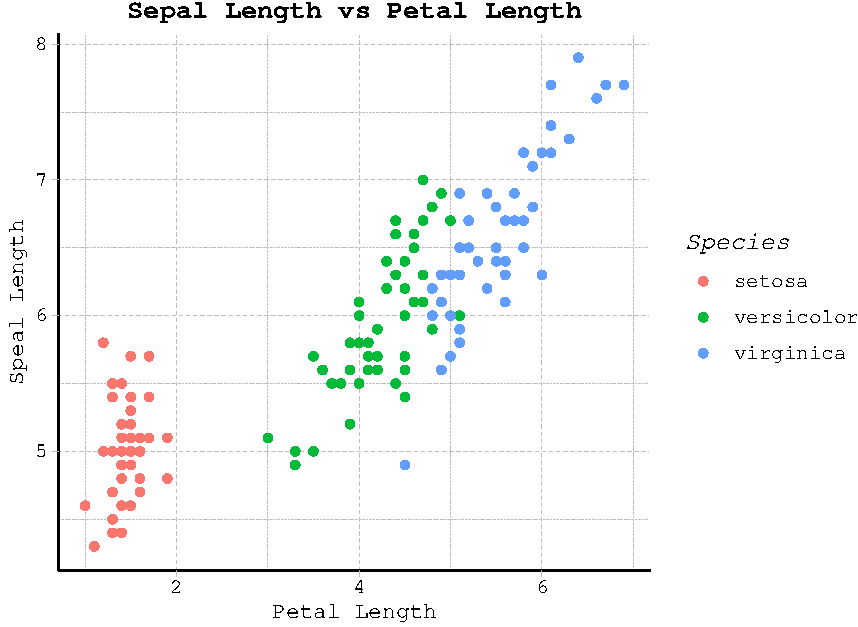
\includegraphics{LR_AIR_Q1_files/figure-latex/unnamed-chunk-5-1.pdf}

Lets make our observations now! As we can see, there seems to be an
overall positive relationship between petal length and sepal length.
Furthermore, the strength of this relationship varies by specie. As for
the sepal and petal lengths, the virginicia has the largest measurements
followed by the versicolor and the setosa.

\newpage

\hypertarget{part-c-multiple-regression}{%
\section{Part c) Multiple Regression}\label{part-c-multiple-regression}}

Our next task is a multiple regression of petal length, petal width and
sepal width on sepal length. Lets see if taking account of these extra
variables changes the relationship exhibited above in the
scatterplot.\newline

\begin{Shaded}
\begin{Highlighting}[]
\KeywordTok{options}\NormalTok{(}\DataTypeTok{scipen =} \DecValTok{3}\NormalTok{) }\CommentTok{# 3 decimal level percision}
\CommentTok{# our model}
\NormalTok{reg <-}\StringTok{ }\KeywordTok{lm}\NormalTok{(Sepal.Length }\OperatorTok{~}\StringTok{ }\NormalTok{Petal.Length }\OperatorTok{+}\StringTok{ }\NormalTok{Petal.Width }\OperatorTok{+}\StringTok{ }\NormalTok{Sepal.Width, iris) }

\CommentTok{# this is the regression output}
\KeywordTok{stargazer}\NormalTok{(reg, }\DataTypeTok{title=}\StringTok{"Multiple Regression Results"}\NormalTok{, }\DataTypeTok{align =} \OtherTok{TRUE}\NormalTok{, }\DataTypeTok{header =} \OtherTok{FALSE}\NormalTok{) }
\end{Highlighting}
\end{Shaded}

\begin{table}[!htbp] \centering 
  \caption{Multiple Regression Results} 
  \label{} 
\begin{tabular}{@{\extracolsep{5pt}}lD{.}{.}{-3} } 
\\[-1.8ex]\hline 
\hline \\[-1.8ex] 
 & \multicolumn{1}{c}{\textit{Dependent variable:}} \\ 
\cline{2-2} 
\\[-1.8ex] & \multicolumn{1}{c}{Sepal.Length} \\ 
\hline \\[-1.8ex] 
 Petal.Length & 0.709^{***} \\ 
  & (0.057) \\ 
  & \\ 
 Petal.Width & -0.556^{***} \\ 
  & (0.128) \\ 
  & \\ 
 Sepal.Width & 0.651^{***} \\ 
  & (0.067) \\ 
  & \\ 
 Constant & 1.856^{***} \\ 
  & (0.251) \\ 
  & \\ 
\hline \\[-1.8ex] 
Observations & \multicolumn{1}{c}{150} \\ 
R$^{2}$ & \multicolumn{1}{c}{0.859} \\ 
Adjusted R$^{2}$ & \multicolumn{1}{c}{0.856} \\ 
Residual Std. Error & \multicolumn{1}{c}{0.315 (df = 146)} \\ 
F Statistic & \multicolumn{1}{c}{295.539$^{***}$ (df = 3; 146)} \\ 
\hline 
\hline \\[-1.8ex] 
\textit{Note:}  & \multicolumn{1}{r}{$^{*}$p$<$0.1; $^{**}$p$<$0.05; $^{***}$p$<$0.01} \\ 
\end{tabular} 
\end{table}

\hypertarget{part-d-interpretation-of-multiple-regression}{%
\subsection{Part d) Interpretation of Multiple
Regression}\label{part-d-interpretation-of-multiple-regression}}

Looking at the above table, we see that, holding petal width and sepal
width constant, a 1 cm increase in petal length is associated with, on
average, a 0.709 cm increase in sepal length. This effect is
statistically significant beyond the 1\% level.

\newpage

\hypertarget{part-e-extra-credit}{%
\section{Part e) EXTRA CREDIT}\label{part-e-extra-credit}}

I would like to see the effect by species. As we saw in the scatter
plot, the relationship is different across species, so lets look at how
different it is.\newline

\begin{table}[!htbp] \centering 
  \caption{Multiple Regression Results with Species} 
  \label{} 
\begin{tabular}{@{\extracolsep{5pt}}lD{.}{.}{-3} } 
\\[-1.8ex]\hline 
\hline \\[-1.8ex] 
 & \multicolumn{1}{c}{\textit{Dependent variable:}} \\ 
\cline{2-2} 
\\[-1.8ex] & \multicolumn{1}{c}{Sepal.Length} \\ 
\hline \\[-1.8ex] 
 Petal.Length & 0.829^{***} \\ 
  & (0.069) \\ 
  & \\ 
 Petal.Width & -0.315^{**} \\ 
  & (0.151) \\ 
  & \\ 
 Sepal.Width & 0.496^{***} \\ 
  & (0.086) \\ 
  & \\ 
 Speciesversicolor & -0.724^{***} \\ 
  & (0.240) \\ 
  & \\ 
 Speciesvirginica & -1.023^{***} \\ 
  & (0.334) \\ 
  & \\ 
 Constant & 2.171^{***} \\ 
  & (0.280) \\ 
  & \\ 
\hline \\[-1.8ex] 
Observations & \multicolumn{1}{c}{150} \\ 
R$^{2}$ & \multicolumn{1}{c}{0.867} \\ 
Adjusted R$^{2}$ & \multicolumn{1}{c}{0.863} \\ 
Residual Std. Error & \multicolumn{1}{c}{0.307 (df = 144)} \\ 
F Statistic & \multicolumn{1}{c}{188.251$^{***}$ (df = 5; 144)} \\ 
\hline 
\hline \\[-1.8ex] 
\textit{Note:}  & \multicolumn{1}{r}{$^{*}$p$<$0.1; $^{**}$p$<$0.05; $^{***}$p$<$0.01} \\ 
\end{tabular} 
\end{table}

R chose the setosa as our base categorical variable. Thus, all else
equal, we see that Versicolors have, on average, a Sepal length that is
0.724 cm smaller than the Setosa and Virginicas have a sepal length that
is, on average, 1.023 cm smaller than the Setoa. The effect of petal
length on predicting speal length is still significant and now predicts
a 0.829 cm increase in sepal length for each 1 cm increase in petal
length, all else equal.

That concludes Q1. The other two questions are done in Python.

\end{document}
